\begin{abstract}
    \noindent A \emph{Haladó gépi tanulás labor} című tárgyra készített projektmunkám témája a gépi tanulási módszerek felhasználásával történő, képek felcímkézésének problémája volt, melyet egy mély neurális háló architektúra segítségével valósítottam meg. A projektmunka során az \emph{Microsoft COCO} adatbázisban található képeket és hozzájuk tartozó címkéket használtam fel. A tanításhoz használt képeket az Inception-v3 konvolúciós hálón előzetesen feldolgoztam, majd egy, a \textit{Bahdanau-figyelem} módszerét implementáló konvolúciós \textit{enkóder} és rekurzív (GRU) \textit{dekóder} szekvenciájából álló  architektúra felhasználásával a hálónak betanítottam. A háló prediktív képességeit mind az eredeti MS COCO adatbázis, tanításhoz nem használt képein, mind pedig általam válogatott képeken teszteltem.
\end{abstract}

\begin{multicols}{2}
\section{Bevezetés} \label{section:1}
A számítógépes látás tudományának alapvető kérdése a digitális képeken szereplő objektumok felismerése, valamint a rajta szereplő cselekmények leírása és kontextusának megértése. Az erre irányuló próbálkozások eredményei első sorban a hardveres, szoftveres, valamint elméleti fejlődésnek köszönhetően, a mély neurális hálók széleskörű alkalmazhatóságának megjelentével lendülhettek nagyban pozitív irányba. Azonban a sikerhez vezető úton való biztos haladáshoz a neurális architektúrák \q{memóriáját} érintő fejlesztések is elengedhetetlennek bizonyultak\citep{yao2014spoken}, melyek a feladat nyelvi, szemantikai részében felmerülő akadályok megugrásában játszanak szerepet. \par
Egy képen szereplő jelenet szemantikus leírásához szükség van mind a képen található jellegzetességek felismerésére, valamint azok alapján értelmes, jó leírásnak nevezhető mondatok létrehozására. A felhasznált algoritmusnak pontosan tisztában kell lennie a szavak nyelvtani rendjével és egy mondat megfogalmazása közben az általa már eddig generált szavakkal és azok jelentésével.
\begin{Figure}
	\centering
	\captionsetup{justification=centering}
	\includegraphics[width=\linewidth]{{img/neural_const.pdf}}
	\captionof{figure}{Az általam alkalmazott háló felépítése}\label{fig:1}
\end{Figure}
\par Ezen meggondolások mentén a projektmunka során egy olyan neurális hálót hoztam létre, mely képes a bemenetként adott képi jelenetet feldolgozni és a rajta látható cselekmény, vagy látkép lényeges részleteit kiemelve, azt egy rövid, \emph{angol nyelvű} mondattal jellemezni. \par
\begin{figure*}[t]
	\captionsetup{justification=centering}
	\includegraphics[width=\textwidth]{{img/sample_images.png}}
	\captionof{figure}{Az adatbázisban található képek egy véletlen mintája. Ezek között szerepelnek mind ún. \emph{ikonikus}, valamint \emph{nem-ikonikus} képek is. Az első típus által jellemzett képek esetén az objektum, vagy leírandó cselekmény kitakarás nélkül, a kép közepén, azt szinte teljesen kitöltve helyezkedik el, ezzel dominálva a jelenetet. Második esetben viszont az objektum esetleg a háttérben található, nem domináns pozícióban.}\label{fig:2}
\end{figure*}
A II. részben a neurális háló tanító- és teszthalmazához felhasznált adatbázisról értekezem részletesebben. A III. fejezetben a háló pontos, véglegesített felépítését tárgyalom, kitérve az általam kipróbált, de kevésbé bevált módszerekre is. Végül a IV. fejezetben a kapott eredményeket és a háló működését szemléltető példákat mutatok be és elemzek, az eddigieket pedig az V. fejezetben diszkutálom.

\section{Felhasznált adatok} \label{section:2}
A projekt során a Microsoft COCO\footnote{COCO: Common Objects in Context}\textsuperscript{,}\footnote{\url{http://cocodataset.org/}}\citep{2014arXiv1405.0312L} (továbbiakban csak \emph{MS COCO}) adatbázisban található képi és címke információkkal dolgoztam. Az adatbázist célirányosan a képi jelenetek leírására, valamint a képeken található objektumok felismerésére törekvő módszerek fejlődését elősegítendő hozták létre. Ahogy az angol elnevezése is utal rá, az adatbázis olyan képek összegyűjtésével jött létre, melyeken átlagosnak mondható, hétköznapi tárgyak, személyek, cselekmények, vagy általánosan közismert jelenetek szerepelnek (\emph{\q{Common Objects...}}), azok természetes környezetében (\emph{\q{...in Context}}). Az adatbázis létének egyik fő célja, hogy elősegítse az olyan objektumok és cselekmények felismerésére törekvő technikák fejlődését, melyek nem csak \emph{ikonikus} jelenetek feldolgozására is alkalmasak. Az MS COCO-ban található képek egy véletlenszerűen választott halmaza a \ref{fig:2}. ábrán látható. \par
Az MS COCO több típusú címkehalmazt tartalmaz, ilyen például a képek szemantikus szempontok alapján történő szegmentálásához, objektumok felismeréséhez vagy éppen a képek kulcsszavakkal, vagy egész mondatokkal történő felcímkézéséhez használható adatok. Ezek közül a projektmunka elkészítéséhez kizárólag a képek egész mondatokkal történő felcímkézéséhez szükséges címkéket használtam. Ebben a kategóriában minden egyes képhez - néhány kivétellel - 5 darab címke tartozik, melyeket egyesével minden kép esetén 5 különböző, független önkéntes fogalmazott meg. Így összesen az adatbázisban található $82783$ darab képhez $414113$ darab címke tartozik jelenleg. \par
Tanítás során az adathalmazt mindig $0,8$-$0,2$-es arányban bontottam tanító, valamint teszthalmazra, így effektíve minden esetben maximálisan csak $331290$ címke, tehát $\approx 66226$ kép felhasználásával tanítottam a neurális hálót.

\section{Technikai részletek} \label{section:3}
Az általam alkalmazott háló nagy részben megegyezik a \textit{Show, Attend and Tell} című cikkben javasolt architektúrával \citep{2015arXiv150203044X}. A projektmunka teljesítéséhez ennek egy kész implementációját vettem a saját munkámhoz alapul, mely a TensorFlow dokumentációinak oldalán szabadon elérhető\footnote{\url{https://www.tensorflow.org/tutorials/text/image_captioning}} és mely kód a TensorFlow 2.0 Python könyvtárban definiált függvényekre épül. Az architektúra felépítésének sematikus reprezentációja az \ref{fig:1}. ábrán látható. \par
Az első szakaszban a tanításhoz használt képek egy enkóder modulon haladnak át, amit egy Inception-v3 háló alkot. Az általam alkalmazott implementációban ez a lépés először lefut a teljes tanítóhalmazon, és a háló kimeneti értékeit külön fájlokba menti. Ennek oka, hogy az MS COCO adathalmaz nagyon nagy, így az enkóder modul teljes kimenete a tanításhoz használt számítógép memóriájába nem férne bele. Ezt megkerülendő - habár a futásidő rovására -, alkalmaztam ezt a bevettnek is nevezhető és javasolt megoldást. A valódi tanítási ciklus során ezek a kimenetek kizárólag már csak egy teljesen kapcsolt rétegen haladnak át a további modulokat megelőzően. \par
Ezt követően egy \q{kemény} Bahdanau-figyelemmel (\emph{hard attention}) felszerelt, GRU típusú dekóder modul következik, mely az \q{erőltetett tanítás} (\emph{teacher forcing}) segítségével generál egymás után következő szavakat a képen szereplő jelenet leírására. Végső lépésként a dekóder meghatározza a modell súlyainak gradiensét és átadja azokat az optimalizálónak a visszaterjesztési lépéshez. \par
A predikció szintén a dekóder modul segítségével történik, azonban ilyenkor már nm alkalmazzuk az erőltetett tanítást a következő szó meghatározására.

\subsection{Tokenizálás}
A dekóder modulban történtek egy klasszifikációs probléma megoldásához is hasonlíthatóak. A dekóder feladata, hogy minden lépésben eldöntse, hogy az általa ismert szavak közül melyik következhet a legnagyobb valószínűséggel a felirat generálása közben, figyelembe véve az eddig már legenerált szavakat és azok jelentését. Ehhez a tanító feliratok felhasználásával, az azokban található egyedi szavakat egy vektorba szétválogatjuk, majd azokat indexeljük, ezt a vektort pedig a továbbiakban \emph{szótár}nak fogom hívni. Minden eredeti képfeliratot a tanítóhalmazban átalakítunk egy fix hosszúságú vektorrá, melyben az egyes szavakat sorrendben a szótárban található indexekkel jelöljük. A fix hosszúságú vektorok azt takarják, hogy minden egyes képfelirathoz tartozó vektor komponenseinek száma, azonosan a leghosszabb felirat hosszával egyenlő. Az aktuális felirat hosszán túllógó komponensek értékeit egységesen $0$-nak választottam. Végül a dekóder modul ezeket a vektorokat kapja az enkóder kimenete mellett bemenetként. \par
A kiindulásként használt kód javaslata alapján a szótár leggyakoribb szavai közül csak az első $5000$ darabot használtam csak fel a tanítás során. A fennmaradó szavak helyére a feliratok vektorrá konvertálása során az \texttt{<unk>} helykitöltő szót helyettesítettem. Az egyes feliratok végének jelzésére az \texttt{<end>} helykitöltőt használtam.

\subsection{Enkóder modul és az Inception-v3}
Az enkóder modul célja a bemeneti képen található fontos részletek kiemelése, azok elraktározása, és a képen szereplő információk minél gazdaságosabb tömörítése. Összefoglalva az enkóder modul a bementi kép fontos tulajdonságait hivatott kiszűrni (\emph{feature extraction}). A számítógépes látás problémáinak megoldásában egyértelműen a konvolúciós lépésekből álló neurális hálózatok használata a legkézenfekvőbb választás és egyben ezek is érik el magasan a legjobb eredményeket a képi információkkal való munkában \citep{khan2018guide}. \par
Az ImageNet képi adatbázis köré szerveződő éves versenyét (\emph{ILSVRC}) \citep{2014arXiv1409.0575R} 2012-ben toronymagasan, az addigi legkorszerűbb módszereket is megverve, az AlexNet nevű konvolúciós neurális háló nyerte meg \citep{krizhevsky2012imagenet}, mely eredmény mind a mesterséges intelligenciával foglalkozó tudományterületek, mind pedig a teljes ipar figyelmét is felkeltette. Az elkövetkezendő években számtalan újabb és egyre jobb konvolúciós neurális architektúra jelent meg, ilyen volt pl. a GoogLeNet \citep{2014arXiv1409.4842S}, a VGG \citep{2014arXiv1409.1556S}, vagy a ResNet \citep{2015arXiv151203385H}. \par
A tanítás során az enkóder modul helyére egy ilyen, korszerűnek nevezhető hálózatot választottam. Választási lehetőségeimet az egyszerűség kedvéért lekorlátoztam a Tensorflow 2.0 könyvtárban már implementált hálózatok csoportjára. A végső választásom az Inception-v3 architektúrára esett, mely a kiindulásként használt kód által javasolva volt, valamint mely az implementált hálók közül talán a legkorszerűbbnek volt nevezhető. Ez a háló a GoogLeNet első megjelenésekor kidolgozott, rendhagyónak látszó, ún. \emph{inception} modulokat használ fel \citep{2015arXiv151200567S}. Az Inception-v3 architektúra jobban teljesít kortársainál az ImageNet adathalmaz képeinek felismerése során, így megfelelő választás az általam megoldandó probléma esetére is. A hálózat felépítése a \ref{table:1}. táblázatban látható.
\begin{center}
\footnotesize
\begin{tabular}{|l|c|r|}
\hline
\textbf{Típus}       & \textbf{Megjegyz.}                      & \textbf{Bemenet}           \\
\hline \hline
conv                 & $3 \times 3 / 2$                        & $299 \times 299 \times 3$  \\ \hline
conv                 & $3 \times 3 / 1$                        & $149 \times 149 \times 32$ \\ \hline
conv padded          & $3 \times 3 / 1$                        & $147 \times 147 \times 32$ \\ \hline
pool                 & $3 \times 3 / 2$                        & $147 \times 147 \times 64$ \\ \hline
conv                 & $3 \times 3 / 1$                        & $73 \times 73 \times 64$   \\ \hline
conv                 & $3 \times 3 / 2$                        & $71 \times 71 \times 80$   \\ \hline
conv                 & $3 \times 3 / 1$                        & $35 \times 35 \times 192$  \\ \hline
$3 \times$ Inception & ld. \cnum{2015arXiv151200567S}, 5. ábra & $35 \times 35 \times 288$  \\ \hline
$5 \times$ Inception & ld. \cnum{2015arXiv151200567S}, 6. ábra & $17 \times 17 \times 768$  \\ \hline
$2 \times$ Inception & ld. \cnum{2015arXiv151200567S}, 7. ábra & $8 \times 8 \times 12803$  \\ \hline
pool                 & $8 \times 8$                            & $8 \times 8 \times 2048$   \\ \hline
\vdots               & \vdots                                  & \vdots                     \\
\end{tabular}
\normalsize
\captionof{table}{Az Inception-v3 hálózat felépítése. Az eredeti architektúrában az utolsó \texttt{pool} réteg után egy \emph{logit} és egy \emph{softmax} függvény is következik.} \label{table:1}
\end{center}
Észrevehető, hogy a táblázatban nem szerepel az eredeti Incenption-v3 hálózat utolsó két rétege, egy \emph{logit}, majd azt követően egy \emph{softmax} függvény. Ennek oka, hogy a Bahdanau-figyelem használata miatt számomra az utolsó Inception modul kimenetére, tehát a táblázatban szereplő utolsó \emph{pool} réteg $(8 \times 8 \times 2048)$-as bemenetére volt szükségem, melyből a képet egy $8 \times 8$ méretű négyzetrácsra felosztva, a rácsközökre végzem a Bahdanau-figyelem műveletét. \par
A képek előzetes feldolgozása során végül ez a $8 \times 8 \times 2048$ méretű kimenet kerül elmentésre. Ez a tenzor egy $(64 \times 2048)$ méretű tenzorrá van összenyomva, amit végül a tanítási lépés során kap meg a meghívandó enkóder modul, amely összesen már csak egy teljesen kapcsolt rétegből (\emph{FC}), valamint ezt követően egy ReLU függvényből áll.

\subsection{Dekóder modul és Bahdanau-figyelem}
Az visszacsatolt neurális hálózatok (\emph{RNN}) enkóder-dekóder modulokra épülő architektúrájában az enkóder feladata a - például - képi bemeneten található fontos információk \q{kódolása}, míg a dekóder modul tulajdonképpen az a tag, amelyik ezen információkból levonható következtetéseket elsődlegesen megtanulja, majd új bemenet esetén abból predikciót képes felállítani. \par
Ahogy a bevezetőben is szerepelt, a szemantikai problémák megoldásában fontos, hogy az általunk implementált neurális háló tisztában legyen a már generált, vagy látott szavak jelentésével és sorrendjével, valamint azok lineáris és globális nyelvtani kohéziójával. A neurális hálók ilyenfajta \q{memóriáját} a visszacsatolt neurális hálók alapvetően képesek megvalósítani, azonban az itt felmerülő eltűnő/felfúvódó gradiensproblémával önmagukban nem tudnak mit kezdeni, mely a gradiensek gyors exponenciális csökkenését, vagy növekedését jelenti. Egy RNN háló továbbá sok esetben képtelen hosszabb adatszekvenciák esetén a szövegben távoli szavak közti összefüggéseket észlelni, így egy hosszabb szövegben levő globális kohéziót bárhogyan is megérteni. Ezen problémák megoldásához többféle módszert is használhatunk, melyek közül az egyik legnépszerűbb a klasszikus RNN cellák helyetti LSTM\footnote{\textbf{L}ong \textbf{S}hort-\textbf{T}erm \textbf{M}emory}, vagy GRU\footnote{\textbf{G}ated \textbf{R}ecurrent \textbf{U}nit} modulok alkalmazása, melyek a háló nagyobb léptékű átalakítása nélkül képesek effektíven megoldani az említett gondokat. \par
A hálózat dekóder része egy, a Bahdanau-figyelem módszerét is implementáló GRU modulokból álló háló. Egy ilyen GRU modul felépítése látható a \ref{fig:3}. ábrán. Az LSTM és GRU közötti választást mindig az adott probléma természete, valamint a rendelkezésre álló számítási kapacitás mennyisége dönti el. Egyes problémák esetén a GRU cellák használata a megfelelő, míg más esetekben az LSTM modulok teljesítenek jobban. Egy GRU cella azonban minden esetben kisebb számítási teljesítményt igényel és így gyorsabb futásidőt jelent, így a jelen projektben ez sokkal inkább számára kedvezett a választásban.
\begin{Figure}
	\centering
	\captionsetup{justification=centering}
	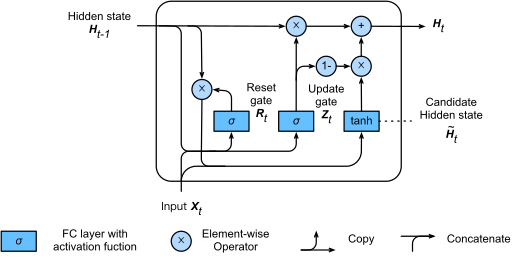
\includegraphics[width=\linewidth]{{img/gru.pdf}}
	\captionof{figure}[Caption of Fig. 3.]{A projektmunka során a hálózatban is implementált GRU cella sematikus ábrája. A kép az online elérhető, nyílt-forrású \emph{Dive into Deep Learning} című könyvből származik\footnotemark.} \label{fig:3}
\end{Figure}
\footnotetext{\url{https://github.com/d2l-ai/d2l-en}}
Mind tanítás, mind pedig tesztképekre adott felirat-generálás közben a minden lépésben meghívott GRU cella 1-1 újabb szót hoz létre, mely lépések során - kialakításából fakadóan - figyelembe veszi az előtte már legenerált szavakat is. A tanítás és a predikció közti egyetlen különbség a tanító fázis során alkalmazott \emph{erőltett tanítás} művelete. Ennek során a sorban következő GRU cella bemeneteként mindig az előző lépésben kapott kimenetet használjunk. Predikció során pedig visszatérünk a szokásos RNN léptetésre. \par
A dekóder modulban a GRU cellával együttesen implementált Bahadanu-figyelem módszere sokat segít a modul pontosságának javításán, mely javulás a hosszabb mondatok esetén még jelentősebbé válik. A figyelem-mechanizmus implementációjának célja a nagyméretű enkóder kimenetből származó információveszteség megelőzése. Az enkóder kimeneti vektora legtöbb esetben nagyon nagy méretű, így a dekóder modulban történő számítások közben egyes fontos információk elveszhetnek, elsikkadhatnak belőle. A Bahdanau által kifejlesztett figyelem-mechanizmus \citep{2014arXiv1409.0473B} abban segít a dekóder modulnak, hogy ebben a sokszor hosszú vektorban melyek azok a pontok és intervallumok, amikre a \emph{figyelmét} szükséges irányítania. A projektmunka során prezentált hálóban az ún. \q{kemény} figyelem módszere van implementálva, mely során a dekóder modul a bemenet csak mindig egy apró, de nagy nagy valószínűséggel fontosnak jelzett szegletére koncentrál erősen.

\section{Eredmények} \label{section:4}
\begin{figure*}[t]
	\captionsetup{justification=centering}
	\includegraphics[width=\textwidth]{{img/sample_predicts.png}}
	\captionof{figure}{A projektmunka során a hálózatot 80 epoch hosszan tanítottam. Az adatbázist $80\%-20\%$ arányban egy tanító- és egy teszthalmazra bontottam, majd tanítás után az eredményeket a teszthalmazból véletlenszerűen választott képeken manuálisan ellenőriztem. Az ábrán néhány véletlenszerűen választott képre adott predikció látható. A háló akkor hagyja abba újabb szavak generálását, amikor az \texttt{<end>} helykitöltőt prediktálja következő szóként a legnagyobb valószínűséggel.}\label{fig:4}
\end{figure*}
A tanítás során az Adam optimalizálót használtam, a veszteségfüggvényt pedig a kategorikus kereszt-entrópia értékének választottam. A tanításhoz konzekvensen minden esetben $80\%-20\%$ arányban osztottam fel a felhasznált adatokat tanítási- és teszthalmazra. A fenti vázolt architektúra esetében azt figyelmet meg, hogy a felhasznált adatok számától függetlenül, a 80. epochnál tovább a háló már számottevően semennyire sem tanul. Kevés adat esetén ekkor a veszteségfüggvény már 0-ra esik le, míg nagyobb mennyiség esetén ugyanezen a ponton túl egy adott veszteségértékhez konvergál. A végleges tanítás veszteségfüggvénye a \ref{fig:5}. ábrán tekinthető meg, ahol ez a konvergáló viselkedés is jól látható.
\begin{Figure}
	\centering
	\captionsetup{justification=centering}
	\includegraphics[width=\linewidth]{{img/loss.png}}
	\captionof{figure}{A végleges beállításokkal, a teljes adatbázisra történő tanítás veszteségfüggvénye. A tanítás 80 epoch hosszan tartott.}\label{fig:5}
\end{Figure}
A feladat természetéből fakadóan sokkal szemléletesebb képet adhat a veszteségfüggvénynél az egyes tesztképekre történő felirat-generálás manuális ellenőrzése. Az előzetes tanítások közben sok, véletlenszerűen választott képre feliratokat generálva, egy kellően átfogó képet kaphatunk a hálózat aktuális teljesítményéről. Ezen tesztek alapján már könnyű volt finomítani a háló beállításain. \par
A végleges háló által generált feliratok egy véletlenszerűen választott csoportja látható a \ref{fig:4}. ábrán. Az eredmények ezzel az architektúrával még nem tökéletesek. A háló láthatóan sok formát még összekever, ilyen pl. az ábrán alsó sorban, balról a második fotó is. A felirat alapján a háló jól felismeri, hogy a képen egy zöld tájképen szereplő objektum szerepel, azonban a templom formáját összetéveszti egy gépkocsiéval. Más esetekben feltehetően pl. a képen látható színek miatt adhat rossz predikciót. Ilyen a felső sorban, jobbról a második kép, ahol a világos, kavicsos talajt hóval téveszti össze. Ebben az esetben azonban a régi gőzmozdonyt és a körbe levő állomást tökéletesen felismeri.

\section{Diszkusszió} \label{section:5}
A projektmunka során sikerült belátnom, hogy a fent vázolt architektúra jó pontossággal képes képi jelenetek és objektumok felismerésére, így a képek feliratozására. Habár a végleges eredmények azt mutatták meg, hogy a háló néha rosszul interpretálja a képen látható alakokat, vagy színeket, azonban még ilyen esetben is logikusan megmagyarázható hibákat követ el. \par
A hálót szinte bármelyik pontján lehetne fejleszteni. Egyik ilyen pl. a \q{kemény} Bahdanau-figyelem helyett egy \q{lágy} figyelem alkalmazása, mely a háló felépítésének alapját megadó \cnum{2015arXiv150203044X} cikkben látottak alapján jobb és pontosabb predikcióra képes. Azonban fejlettebb és korszerűbb enkóder modulok használata is javulást eredményezhet a véglegesen kapott eredményekben.
\end{multicols}